\section{Commercial success: funding, listing, and the firms that mattered}\label{sec:success}

A mark that survived the five-year proof names a product that held its
place in commerce. This section asks whether the owners of leading or
atypical debut filings went on to the outcomes that make a firm rich: a
priced private round, SEC financial reporting, a public listing, and
revenue at scale. The unit is the owner's first registered filing, its
debut, scored on the production measure; the outcomes are dated events in
the SEC record. Form D became mandatory in electronic form on 16 March
2009, so the funding ladder is built on debuts made 2009--2018, for which
every rung is observed; the public-reporting analysis uses the longer
1995--2018 sample.

\subsection{The ladder: a round, reporting, a listing}\label{sec:ladder}

Of 999{,}442 owners whose first registered filing, carrying a score, was
made 2009--2018, 17{,}115 (1.71\%) raised a priced private round after the
debut, 4{,}383 (0.44\%) appear in SEC reporting records at any time, and
1{,}795 (0.18\%) registered a class of securities or completed an initial
public offering at any time. The funded rung requires the round to
postdate the debut; the reporting and listing rungs do not, so owners
already reporting before their first trademark filing are counted, and the
staged analysis in Section~\ref{sec:discussion} shows they are a majority
of the exchange-listed. The rungs nest: 7.3\% of funded owners reach
reporting against 0.3\% of the unfunded, and 41\% of reporting owners
reach an IPO.

Table~\ref{tab:ladder} gives the rate at each rung by fifth of lead and of
atypicality, with fifths cut within Nice class, debut year, and fifth of
description length, so that neither the industry, the year, nor the length
of the description enters the contrast. Funding does not vary with either
axis: the most leading fifth of debuts is funded at 1.80\% against 1.86\%
for the most lagging, and the most atypical at 1.64\% against 1.68\%, both
inside sampling error. Trademark counts and breadth carry a funding signal
\citep{Block2014}; vocabulary position does not. Reporting and listing do
vary. Owners whose debut language was most lagging reach reporting at
0.59\%, owners whose debut language was most leading at 0.38\%; for an IPO
the rates are 0.24\% and 0.17\%. On atypicality the sign is positive on
this sample: the most atypical fifth reports at 0.53\% against 0.42\% for
the most conventional, and lists at 0.22\% against 0.15\%.
Section~\ref{sec:bluesea} absorbs description length continuously on
1995--2018 debuts and finds the atypicality gradient flat; with length
held in fifths on 2009--2018 debuts it is positive at $t$ above 4. The two
are stated side by side; the difference between them is a length control
and a sample, and the atypicality result at the listing margin is the one
claim in the paper that depends on which is used.

\begin{table}[h]\centering\small
\caption{The ladder by fifth of debut lead and of debut atypicality. Rates
in percent of owners whose first registered filing was made 2009--2018
($n = 999{,}442$); fifths cut within Nice class, debut year, and fifth of
description length. The last column is the most-minus-least contrast with
its $t$-statistic.}
\label{tab:ladder}
\begin{tabular}{llrrrrrr}
\toprule
Rung & Axis & Q1 & Q2 & Q3 & Q4 & Q5 & Q5$-$Q1 (pp; $t$) \\
\midrule
Funded    & lead         & 1.86 & 1.73 & 1.61 & 1.57 & 1.80 & $-0.06$ ($-1.4$) \\
          & atypicality  & 1.68 & 1.70 & 1.79 & 1.76 & 1.64 & $-0.04$ ($-1.1$) \\
Reporting & lead         & 0.59 & 0.49 & 0.40 & 0.34 & 0.38 & $-0.21$ ($-9.4$) \\
          & atypicality  & 0.42 & 0.36 & 0.43 & 0.46 & 0.53 & $+0.11$ ($+5.2$) \\
IPO       & lead         & 0.24 & 0.21 & 0.14 & 0.13 & 0.17 & $-0.07$ ($-4.5$) \\
          & atypicality  & 0.15 & 0.15 & 0.18 & 0.21 & 0.22 & $+0.07$ ($+4.8$) \\
\bottomrule
\end{tabular}
\end{table}

The lead profile at reporting and at IPO is not monotone: it falls from
the lagging end through the fourth fifth and turns up in the fifth. Owners
whose first description used language the class was leaving behind are the
likeliest to report and to list. Most of them are established firms making
a first trademark filing late in a business already built on the class's
older vocabulary, and the ladder cannot separate that from anything the
language itself does. Listings that arrive without an observed post-debut
Form~D round lean the same way: their owners' debut lead averages $-0.25$
standard deviations against $-0.08$ for funded listings --- consistent
with established, revenue-financed businesses listing without venture
money, where ``unfunded'' means only that no Form~D notice is observed.

\subsection{The firms that produced the most value}\label{sec:value}

Among the 1.80 million owners whose first registered filing was made
1995--2018, 4{,}710 link to SEC financial statements with reported
revenue; ten of them hold 18.5\% of the \$19.2 trillion of linked peak
revenue and five hundred hold 82.9\%. Reading this handful is not a
statistical argument, but it is not a stray anecdote either: these are
the firms in which most of the linked value was generated, and their
debut language was ordinary --- the ten largest sit $0.35$ standard
deviations \emph{below} average atypicality and within $0.01$ of average
lead, and the revenue-weighted linked set sits at the average on both
axes (tier detail in the supplementary material). Hand-curated
vocabularies sharpen the same point from the other side: debuts in AI or
blockchain vocabulary are funded four to five times as often as the
average debut (7.8\% and 8.4\% against 1.7\%), but reach reporting and
listing only about twice as often, on small counts (supplementary
material).

\subsection{Leading debuts reach public reporting less often; unusual ones no more often}\label{sec:bluesea}

The outcome here is whether an owner ever appears in the Securities and
Exchange Commission's financial reporting records. That is broader than
exchange-listed: roughly half the matched firms carry a ticker and the
rest report for other reasons. Figure~\ref{fig:successcurves} draws the
raw rate against each axis in twenty bins. In signed lead the profile is a
U whose tails both sit above the base rate and whose lagging tail is the
higher; in lead magnitude and in atypicality the raw rate rises.

\begin{figure}[h]\centering
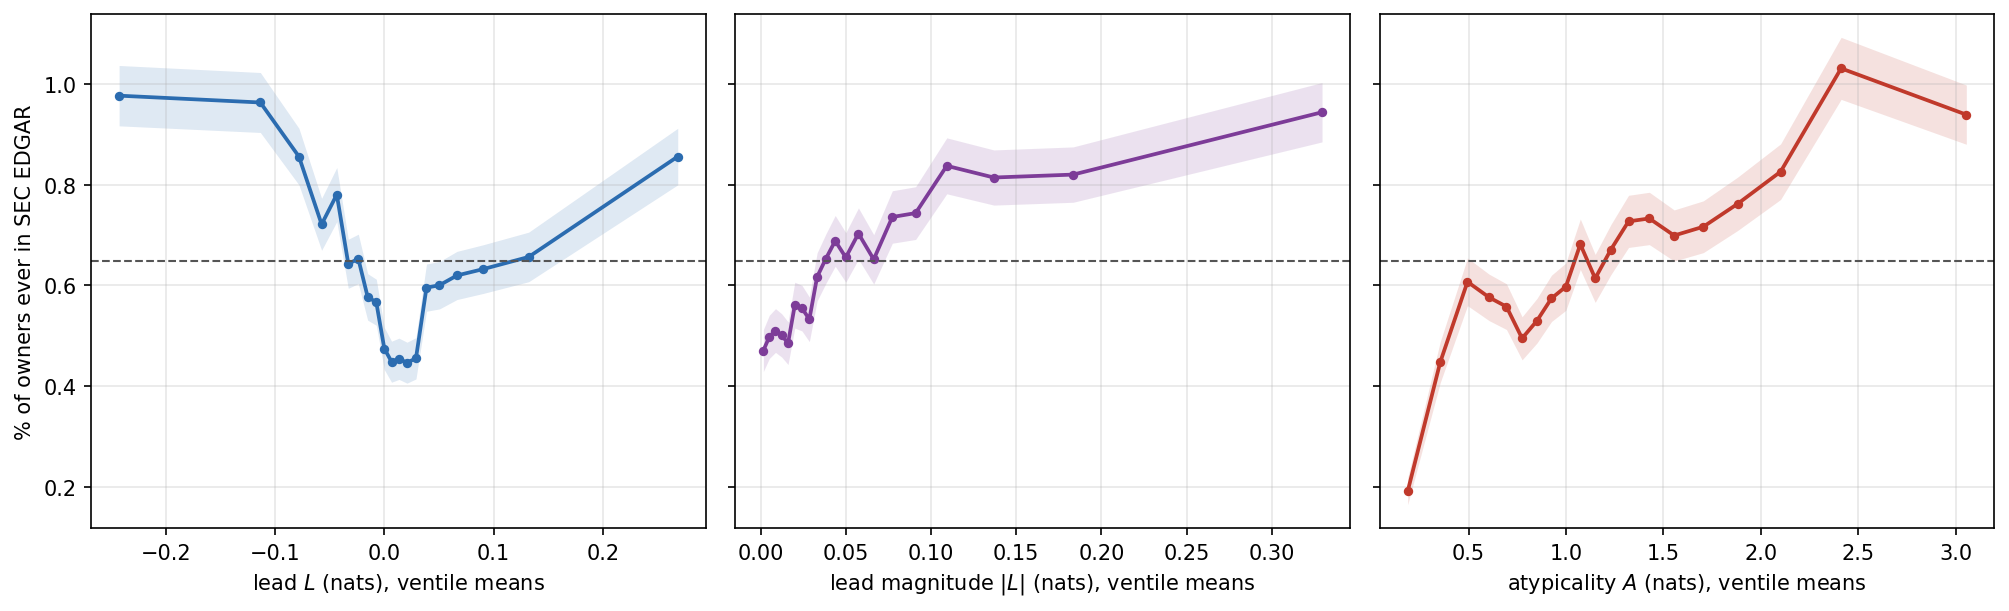
\includegraphics[width=\textwidth]{results/fig_success_ventiles.png}
\caption{Share of registered debut owners (first registered filing
1995--2018, $n = 2{,}066{,}600$) ever appearing in SEC EDGAR, in twenty
equal-count bins of debut lead $L$, lead magnitude $|L|$, and atypicality
$A$, cut on the pooled distribution. Bands are 95\% binomial intervals;
the dashed line is the 0.65\% base rate. These are raw rates carrying
class, year and length composition; Table~\ref{tab:edgar} gives the
design-based estimates, under which the atypicality gradient is absorbed
and the signed-lead U remains.}
\label{fig:successcurves}
\end{figure}

The raw atypicality gradient does not survive the design-based estimates
(Table~\ref{tab:edgar}). Within class and filing year, holding description
length fixed, top-quintile atypicality raises the probability of SEC
reporting by $+0.000$pp on a 0.481\% base ($t = 0.0$), and by $-0.003$pp
on the past level alone. The quintile profile is not even monotone: the
three middle quintiles sit \emph{below} the bottom one and the top merely
returns to it. The 2.7-fold gradient in the raw bins is composition:
firms that go on to report cluster in particular classes, years, and
multi-class filings, and class$\times$year fixed effects absorb it. Lead
costs, at equal atypicality: the signed component enters negatively
($-0.047$pp per standard deviation, $t = -7.8$) while the unsigned
component enters positively ($+0.067$pp per standard deviation,
$t = 7.7$). The U in the raw bins is exactly this pair: lagging filings
show the magnitude premium with no lead penalty, leading filings show it
net of that penalty, and the middle bins show neither. Once the levels
are controlled, the recovery of the far-leading tail is much reduced: the
quintile profile falls through Q4 and recovers only slightly at Q5.

\begin{table}[h]\centering\small
\caption{Debut listing and vocabulary position: design-based estimates.
LPM of P(owner ever in SEC EDGAR) on 1{,}556{,}968 registered debut
filings 1995--2018, one observation per owner, class$\times$filing-year
fixed effects, heteroskedasticity-robust SEs. Quintiles cut within
class$\times$year. Base rate 0.481\%.}
\label{tab:edgar}
\begin{tabular}{lrr}
\toprule
 & Coefficient (pp) & SE \\
\midrule
\multicolumn{3}{l}{\emph{Atypicality quintiles, $A = \tfrac{1}{2}(K^{-}+K^{+})$ (Q1 omitted)}} \\
\quad Q5, FE only & $+0.017$ & $0.018$ \\
\quad Q5, FE + log length & $+0.000$ & $0.018$ \\
\quad Q5, FE + log length, on $K^{-}$ alone & $-0.003$ & $0.018$ \\
\midrule
\multicolumn{3}{l}{\emph{Signed lead quintiles, FE + log length + KL levels}} \\
\quad Q3 & $-0.133$ & $0.020$ \\
\quad Q4 & $-0.187$ & $0.021$ \\
\quad Q5 & $-0.158$ & $0.024$ \\
\midrule
\multicolumn{3}{l}{\emph{Decomposition, FE + log length}} \\
\quad lead magnitude $|L|$ (pp per sd) & $+0.067$ & $0.009$ \\
\quad signed lead $L$ (pp per sd) & $-0.047$ & $0.006$ \\
\quad log description length & $+0.056$ & $0.004$ \\
\bottomrule
\end{tabular}
\\[0.3em]\footnotesize Standard errors in place of significance stars; see
the note to Table~\ref{tab:gate_lpm}.
\end{table}

Owners are matched to SEC registrants by normalized exact name, over a
candidate universe of all 5.67 million owners in the corpus; names
resolving to more than one registrant are dropped rather than assigned,
and one match is kept per owner string. That yields 19{,}889 matched
owners covering 7{,}588 registrants, and a base rate of 0.481\% among
registered debut filers. Validation on 22 companies that indisputably went
public --- across software, pharmaceuticals, food, apparel, aerospace and
autos --- matches all 22. A random sample of 25 matches carrying at least
three filings was inspected by hand and none was wrong, which is a check
on gross failure modes rather than a precision estimate.

The linkage is nonetheless a name match, and that bounds the atypicality
reading in particular. Firms with distinctive names are easier to match
than firms with generic ones, and distinctiveness of a name plausibly
travels with distinctiveness of the goods/services text; nothing in this
design separates the two. The lead coefficient is unchanged under
alternative linkages; the atypicality coefficient is not, so only the
lead result is robust to the name-match design. The financing rows of
Table~\ref{tab:staged} rest on a Form~D match whose raw extracts are not
in the current tree and should be read as provisional.

The U is also not atypicality working through lead's construction (the
mechanical coupling stated in Section~\ref{sec:three_scorings}): on this
sample lead magnitude and atypicality correlate at $+0.25$, signed lead at
only $-0.10$, and cutting lead fifths within fifths of atypicality keeps
the structure: the most lagging fifth out-reports the most leading in four
of the five atypicality strata (by $0.08$ to $0.39$pp on sub-1\% bases),
and the ordering reverses only in the most atypical fifth, where the most
leading debuts report most. The lagging tail's premium is not a ceiling
artifact; the leading tail's partial recovery in the raw U is where the
atypicality composition lives, which is what the level controls in
Table~\ref{tab:edgar} absorb.

``SEC reporting'' is not ``went public'': splitting matched owners on
whether their SEC filer number carries a ticker gives $10{,}556$ listed
against $9{,}333$ reporting without one, and both halves show the same U
in lead (Section~\ref{sec:robust}), so the result is not an artifact of
counting non-operating registrants as successes.

\subsection{The construct is not patenting}\label{sec:patent}

Within the firms that do both, trademark vocabulary and patenting move
independently. On a panel of trademark owners name-matched to PatentsView
patent assignees \citep{PatentsView}, each axis is regressed on
$\log(1 + \mathrm{patents})$ with firms absorbed and errors clustered on
the firm, estimated on 94{,}181 firm-years across 17{,}506 firms under
theme scoring (93{,}551 and 17{,}415 under term scoring) --- 134{,}075
matched firm-years before dropping the firm-years that contribute no
within-firm variation. The outcome is standardized, so $\beta$ is the
shift in standard deviations of the axis per unit of log-patents; one
unit is roughly a tripling of the patent count, and a firm going from
none to twenty moves about three units.

\begin{center}\small
\begin{tabular}{llrrr}
\toprule
Text counted as & Axis & $\beta$ (sd) & $t$ & Between-firm $r$ \\
\midrule
Themes & atypicality & $+0.012$ & $+3.0$ & --- \\
Themes & lead        & $-0.058$ & $-9.4$ & $-0.020$ \\
Terms  & atypicality & $-0.055$ & $-11.5$ & --- \\
Terms  & lead        & $+0.012$ & $+2.0$ & --- \\
\bottomrule
\end{tabular}
\end{center}

\noindent The grid is close to a mirror: whichever axis carries the small
signal under one way of counting the text carries the opposite sign under
the other. The theme-scored \emph{lead} coefficient ($-0.058$) and the
term-scored \emph{atypicality} coefficient ($-0.055$) are nearly the same
number attached to different quantities. Only those two cells are
established; the mirror's other diagonal is within noise, and the
orthogonality conclusion rests on the magnitude bound --- every cell
under $0.06$ standard deviations --- rather than on any cell's sign.
Nothing here reaches a tenth of a standard deviation.

One objection is timing: a patent is applied for before its invention is
in public use and a trademark when the firm is ready to sell, so patents
would lead. Firms do not proceed that linearly \citep{Seip2018}, and no
timing offset from $t-2$ to $t+1$ isolates a direction ($-0.054$ to
$-0.089$ sd under theme scoring, $+0.012$ to $+0.024$ under terms);
among owners who both patent and raise a priced round, neither event
systematically precedes the other (median lag zero years).

The second objection is heterogeneity: a pooled near-zero could hide a
positive slope where the two rights are complements offsetting a negative
one where trademarks work alone. On a coarse, judgement-based sorting of
classes into complements and substitutes --- assigned in advance from the
class definitions, nothing estimated --- the slopes are $-0.000$ among
complements, $-0.026$ among substitutes, interaction $-0.008$
($t = -0.49$), and the complement classes do not agree in sign with one
another (cell detail in the supplementary material). Neither retention
supports the complementarity story, with the caveats that a coarse
sorting can miss a finer-grained one and that conditioning on a
successful assignee match pushes any interaction toward zero.

\subsection{Leading does not pay, even where novelty does}\label{sec:success_conclusion}

The answer to this section's question is no. An owner whose surviving
product had been described ahead of its industry's language is not more
likely to raise a priced round, reaches SEC reporting and listing
\emph{less} often than a lagging owner, and is absent from the top of the
linked revenue distribution, whose firms debuted in ordinary language.
What pays at the reporting margin is unsigned: lead magnitude and
description length, the marks of a specific, seriously drafted first
filing, carry positive coefficients while the signed component stays
negative. Being unusual is at worst free and at best mildly rewarded;
having been early is never rewarded at any rung the record shows, and
the listings that arrive without observed venture money belong
disproportionately to the lagging.
